
\chapter{Matematický model}
\label{chap:MatMod}

\pagestyle{plain}

    M\v{e}jme trojrozm\v{e}rnou oblast $\Omega \subset{\mathbb{R}^3}$ s hranic\'{\i} $\partial \Omega$. V t\'{e}to oblasti uva\v{z}ujeme pevn\'{e} t\v{e}leso $\Omega_b \subset{\Omega}$. \v{C}asov\'{y} interval uva\v{z}ujme $\mathcal{I} = \langle0,\mathcal{T} \rangle \subset{\mathbb{R}}$ pro $\mathcal{T}>0$.

    % Jako v\'{y}po\v{c}etn\'{\i} oblast budeme ch\'{a}pat oblast ${\Omega} \subset {\mathbb{R}^3}$, uvnit\v{r} kter\'{e} um\'{\i}st\'{\i}me pevn\v{e} t\v{e}leso ${\Omega}_{b} \subset {\Omega}$, viz~obr\'{a}zek \ref{fig:domain1-1}. D\'{a}le uva\v{z}ujeme \v{c}asov\'{y} interval $\mathcal{I} = \langle0,T\rangle \subset{\mathbb{R}}$ pro $T>0$. Rovnice popisuj\'{\i}c\'{\i} dynamiku tekutin pop\'{\i}\v{s}eme v $\mathbb{R}^{3}$, p\v{r}i implementaci 2D \'{u}lohy budeme uva\v{z}ovat t\v{r}et\'{\i} rozm\v{e}r jako jednotkov\'{y}.

    % \begin{figure}[H]
    %     \centering
    %     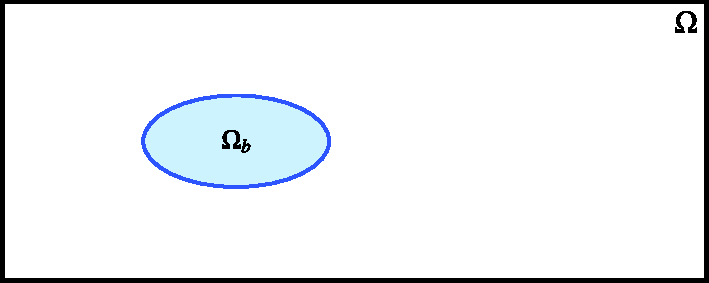
\includegraphics{Img/Kapitola1/domain1-1.pdf}
    %     \caption{Dvourozm\v{e}rn\'{a} v\'{y}po\v{c}etn\'{\i} oblast $\Omega$ s t\v{e}lesem $\Omega_b$ um\'{\i}st\v{e}n\'{y}m uvnit\v{r} oblasti.}
    %     \label{fig:domain1-1}
    % \end{figure} 
    
    \section{Popis dynamiky tekutiny}
    \label{sec:DesFluDyn}
        
        K popisu tekutin chceme pou\v{z}\'{\i}t diferenci\'{a}ln\'{\i} po\v{c}et. To lze za p\v{r}edpokladu, \v{z}e p\v{r}i makroskopick\'{e}m pohledu m\r{u}\v{z}eme tekutinu pova\v{z}ovat za spojit\'{e} prost\v{r}ed\'{\i} (kontinuum), ve kter\'{e}m zanedb\'{a}v\'{a}me \v{c}\'{a}sticov\'{e} vlastnosti tekutin. To plat\'{\i} i pro infinitezim\'{a}ln\v{e} malou \v{c}\'{a}st kontinua. Pro tekutinu tedy dost\'{a}v\'{a}me Navierovy-Stokesovy-Fourierovy rovnice v konzervativn\'{\i}m tvaru popisuj\'{\i}c\'{\i} dynamiku tekutiny
        \begin{subequations}
        \label{eq:NSequ}
        \begin{align}
            \frac{\partial \rho}{\partial t} + \nabla \cdot (\rho \boldsymbol{u}) &= 0, 	\label{eq:ConEqu} \\    
            \frac{\partial (\rho u_i)}{\partial t} + \nabla \cdot (\rho u_i \boldsymbol{u}) &= - \frac{\partial p}{\partial x_i} + \frac{\partial \tau_{i1}}{\partial x_1} + \frac{\partial \tau_{i2}}{\partial x_2} + \frac{\partial \tau_{i3}}{\partial x_3} + \rho F_i, \ i \in \{1,2,3\}, \label{eq:LawConMom} \\
            \frac{\partial}{\partial t}\left[\rho\left(E + \frac{\boldsymbol{u}^2}{2}\right)\right] + \nabla \cdot \left[\rho\left( E + \frac{\boldsymbol{u}^2}{2}\right)\boldsymbol{u}\right] &= \nabla \cdot (\kappa \nabla T) + \rho \boldsymbol{F} \cdot \boldsymbol{u} + \rho Q + \sum_{k=1}^{3}\frac{\partial}{\partial x_k}\left(\sum_{i=1}^{3}u_i\tau_{ik}\right) - \nabla \cdot (\rho \boldsymbol{u}), \label{eq:LawConPotEne}
        \end{align}    
        \end{subequations}
        
        kde $\rho = \rho(\boldsymbol{x},t, T) \ [\mathrm{m \; s^{-3}}]$  je hustota tekutiny, $\boldsymbol{u} = \boldsymbol{u}(\boldsymbol{x},t) \ [\mathrm{m \; s^{-1}}]$ zna\v{c}\'{\i} vektor rychlosti pro $\boldsymbol{x} \in \Omega \ [\mathrm{m}]$, $t \in \mathcal{I} \ [ \mathrm{s}]$, $p = p(\boldsymbol{x},t, T) \ [\mathrm{kg \; m^{-1} \; s^{-2}}]$ vyjad\v{r}uje tlak okoln\'\i ho materi\'alu, $\boldsymbol{F} = \boldsymbol{F}(\boldsymbol{x},t, T) \ [\mathrm{kg \; m \; s^{-2}}]$ je objemov\'a s\'\i la vzta\v{z}en\'a na jednotku hmotnosti a dynamick\'y tenzor nap\v{e}t\'{\i} zna\v{c}\'{\i}me $\boldsymbol{T}_D = (\tau_{ij}) \ [ \mathrm{kg \; m^{-1} \; s^{-2}}]$. D\'ale $E = E(\boldsymbol{x},t, T) \ [\mathrm{kg \; m^{2} \; s^{-2}}]$ vyjad\v{r}uje specifickou vnit\v{r}n\'i energii, $\kappa  \ [\mathrm{kg \; m \; K^{-1} \; s^{-3}}]$ se naz\'yv\'a koeficient tepeln\'e vodivosti, $T = T(\boldsymbol{x},t) \ [\mathrm{K}]$ je teplota tekutiny  a $Q = Q (\boldsymbol{x},t) \ [\mathrm{kg \; m^{2} \; s^{-3}}]$ je hustota tepeln\'{y}ch zdroj\r{u} na jednotku hmotnosti.
        
        Tekutinu uva\v{z}ujeme newtonovskou, tud\'{\i}\v{z} slo\v{z}ky dynamick\'eho tenzoru nap\v{e}t\'{\i}, viz \cite{landau2013fluid}, jsou pro $i, j~\in~\{ 1{,}2{,}3 \}$ ve tvaru
        
        \begin{equation}
        \label{eq:DynStrTen-a}
            \tau_{ij} = \lambda\nabla \cdot \boldsymbol{u} + 2\mu\frac{\partial u_i}{\partial x_i} \qquad i = j,
        \end{equation}
        \begin{equation}
        \label{eq:DynStrTen-b}
            \tau_{ij} = \tau_{ji} = \mu\left(\frac{\partial u_i}{\partial x_j} + \frac{\partial u_j}{\partial x_i}\right) \qquad i \neq j,
        \end{equation}
        kde $\mu \ [\mathrm{kg \; m^{-1} \; s^{-1}}]$ se naz\'yv\'a sou\v{c}initel molekul\'arn\'{\i} viskozity nebo tak\'e dynamick\'a viskozita a plat\'{\i} $\mu = \rho \nu$, pro kinematickou viskozitu $\nu \ [\mathrm{m^{2} \; s^{-1}}]$. Ve vztahu \eqref{eq:DynStrTen-a} se objevuje tak\'{e} druh\'y visk\'ozn\'{\i} koeficient $\lambda \ [\mathrm{ kg \; m^{-1} \; s^{-1} ]}$, pro kter\'y uva\v{z}ujeme Stokesovu hypot\'ezu \cite{buresti2015note}
        
        \begin{equation}
        \label{eq:StoHyp}
            \lambda = - \frac{2}{3}\mu. 
        \end{equation}
        

    \section{Veden\'{\i} tepla}
    \label{sec:HeatTransfer}

        Rovnici pro z\'{a}kon zachov\'{a}n\'{\i} energie \eqref{eq:LawConPotEne} zjednodu\v{s}\'{\i}me pomoc\'{\i} rovnice veden\'{\i} tepla. Celkov\'{a} zm\v{e}na tepeln\'{e} energie za \v{c}as je rovna tepeln\'{e}mu toku p\v{r}es hranici $\varphi \ [\mathrm{kg \; s^{-3}}]$ a tepeln\'{e} energii generovan\'{e} vn\v{e}j\v{s}\'{\i}mi zdroji $Q$. To lze symbolicky zapsat jako
        \begin{equation}
            \label{eq:HeaEquFir}
            \frac{\partial}{\partial t}\left(\rho c T\right) = - \nabla \cdot \left( \varphi + \rho  cT \boldsymbol{u} \right) + Q,
        \end{equation}
        kde $c \ [\mathrm{m}^{2} \ \mathrm{s}^{-2} \ \mathrm{K}^{-1}]$ je m\v{e}rn\'{a} tepeln\'{a} kapacita. Tepeln\'{y} tok $\varphi$ je z Fourierova z\'{a}kona definov\'{a}n vztahem 
        \begin{equation}
            \label{eq:HeaFlu}
            \varphi = - \kappa \nabla T,
        \end{equation}
        kde $\kappa = \kappa ( \boldsymbol{x}) \ [\mathrm{kg \; m \; s^{-3} \; K^{-1}}]$ vystupuje v roli sou\v{c}initele tepeln\'{e} vodivosti a $\nabla T \ [\mathrm{K \; m^{-1}}]$ ozna\v{c}uje teplotn\'{\i} gradient. P\v{r}edpokl\'{a}dejme, \v{z}e hustota $\rho$ je konstantn\'{\i}. Dosazen\'{\i}m \eqref{eq:HeaFlu} do \eqref{eq:HeaEquFir} dostaneme
        \begin{equation}
            \label{eq:HeaEqu1}
            \frac{\partial (cT)}{\partial t} = \frac{1}{\rho} \nabla \cdot ( \kappa \nabla T ) - \nabla \cdot ( cT \boldsymbol{u} ) + \frac{Q}{\rho}.
        \end{equation}
        V p\v{r}\'{\i}pad\v{e}, \v{z}e $\kappa$ a $c$ jsou tak\'{e} konstantn\'{\i}, lze tuto rovnici p\v{r}epsat do tvaru
        \begin{equation}
            \label{eq:HeaEqu}
            \frac{\partial T}{\partial t} = D \Laplace T - \boldsymbol{u}\cdot \nabla T + \frac{Q}{\rho c},
        \end{equation}
        kde jsme ozna\v{c}ili difuzn\'{\i} koeficient $D = \frac{\kappa}{\rho c} \ [\mathrm{m^{2} \; s^{-1}}]$ a Laplace\r{u}v oper\'{a}tor $\Laplace = \nabla \cdot \nabla$.
        
        Pro p\v{r}estup tepla zav\'{a}d\'{\i}me sou\v{c}initel p\v{r}estupu tepla $\omega \ [ \mathrm{kg \ s^{-3} K^{-1}}]$
        \begin{equation}
            \label{eq:TranCoef}
            \omega = \frac{\varphi}{\Delta T},
        \end{equation}
        kde $\Delta T$ ozna\v{c}uje rozd\'{\i}l teplot na rozhran\'{\i} mezi t\v{e}lesem a p\v{r}ek\'{a}\v{z}kou.

        % \subsection{Veden\'{\i} tepla konvekc\'{\i}}    
        
        % Nucen\'{a} vs. Voln\'{a}
        
        
        
        
        % \subsection{Veden\'{\i} tepla kondukc\'{\i}}


    \section{Charakteristick\'e veli\v{c}iny}
    \label{sec:ChaVal}
        
        P\v{r}i popisu proud\v{e}n\'{\i} tekutin je dobr\'{e} zav\'{e}st n\v{e}kter\'{e} veli\v{c}iny, kter\'{e} pomohou b\v{e}hem n\'{a}sledn\'{e}ho vyhodnocov\'{a}n\'{\i} v\'{y}sledk\r{u} l\'{e}pe charakterizovat jednotliv\'{e} typy proud\v{e}n\'{\i} tekutin, viz \cite{ruzicka2008dimensionless}. Mezi tyto veli\v{c}iny pat\v{r}\'{\i}:
        \begin{itemize}
            \item Reynoldsovo \v{c}\'{\i}slo \begin{equation}
                \label{eq:ReyNum}
                    \mathrm{Re} = \frac{l_{0}^{2}}{t_{0}\nu} = \frac{l_{0}u_{0}}{\nu},
                \end{equation}
            % \item P\'{e}cletovo \v{c}\'{\i}slo \begin{equation}
            %     \label{eq:PecNum}
            %         \mathrm{Pe} = \frac{l_{0}^{2}}{t_{0}\nu} = \frac{l_{0}u_{0}}{\alpha},
            %     \end{equation}
            % \item Rayleighovo \v{c}\'{\i}slo \begin{equation}
            %     \label{eq:RayNum}
            %         \mathrm{Ra} = \frac{l_{0}^{2}}{t_{0}\nu} = \frac{l_{0}u_{0}}{\alpha},
            %     \end{equation}
            \item Sherwoodovo \v{c}\'{\i}slo \begin{equation}
                \label{eq:SheNum}
                    \mathrm{Sh} = \frac{\omega l_{0}}{D_{0}} = \frac{k}{u_0},
                \end{equation}
            \end{itemize}
        kde $\omega$ je koeficient p\v{r}estupu a $l_0, t_0, u_0, D_0$ zna\v{c}\'{\i} po \v{r}ad\v{e} charakteristickou d\'{e}lku, \v{c}as, rychlost a difuzi.
            
        
        % \subsection{Reynoldsovo číslo}
        % \label{sub:ReyNum}

        %     Pro popis dynamiky tekutin je v\'{y}hodn\'{e} pou\v{z}\'{\i}t bezrozm\v{e}rn\'{y} popis veli\v{c}in. Pro p\v{r}evody mezi syst\'{e}my jednotek se pou\v{z}\'{\i}v\'{a} Reynoldsovo \v{c}\'{\i}slo, bezrozm\v{e}rn\'{a} veli\v{c}ina definovan\'{a} vztahem 
            
        %     \begin{equation}
        %     \label{eq:ReyNum}
        %         \mathrm{Re} = \frac{l_{0}^{2}}{t_{0}\nu} = \frac{l_{0}u_{0}}{\nu},
        %     \end{equation}
        %     kde $l_{0}$ $[\mathrm{m}]$ je charakteristick\'{a} d\'{e}lka, kter\'{a} je pro simulace v\v{e}t\v{s}inou volena jako jeden z rozm\v{e}r\r{u} oblasti $\Omega$ nebo $\Omega_b$, d\'{a}le $u_{0}$ $[\mathrm{m \ s^{-1}}]$ je charakteristick\'{a} rychlost a $t_{0}$ $[\mathrm{s}]$ je charakteristick\'{y} \v{c}as spl\v{n}uj\'{\i}c\'{\i} vztah $t_{0} = \frac{l_{0}}{u_{0}}$. Rychlost $u_{0}$ vol\'{\i}me jako maxim\'{a}ln\'{\i} nebo pr\r{u}m\v{e}rnou rychlost p\v{r}edepsanou ve v\'{y}po\v{c}etn\'{\i} oblasti $\Omega$. 
            
            % P\v{r}i implementaci m\v{r}\'{\i}\v{z}kov\'{e} Boltzmannovy metody p\v{r}ejdeme za pomoci Reynoldsova \v{c}\'{\i}sla od fyzik\'{a}ln\'{\i}ch jednotek k bezrozm\v{e}rn\'{y}m. P\v{r}i p\v{r}evodu vyu\v{z}ijeme principu podobnosti, tj. vlastnosti Reynoldsovo \v{c}\'{\i}sla, \v{z}e jeho hodnota z\r{u}st\'{a}v\'{a} v obou syst\'{e}mech stejn\'{a}, viz \cite{reynolds1883xxix}.
    % \section{Chlad\'{\i}c\'{\i} syst\'{e}m FSE.12}

    %     V t\'{e}to \v{c}\'{a}sti pop\'{\i}\v{s}eme chlad\'{\i}c\'{\i} syst\'{e}m elektrick\'{e} formule FSE.12. Chlad\'{\i}c\'{\i} syst\'{e}m FSE.12 sest\'{a}v\'{a} ze dvou odd\v{e}len\'{y}ch okruh\r{u} (lev\'{e}ho a prav\'{e}ho), kde ka\v{z}d\'{y} z okruh\r{u} m\'{a} za \'{u}kol odv\'{e}st teplo z celkem t\v{r}\'{\i} komponent: ze dvou motor\r{u} (p\v{r}edn\'{\i}ho a zadn\'{\i}ho -- um\'{\i}st\v{e}ny v kolech) a z m\v{e}ni\v{c}\r{u}. Samotn\'{y} chlad\'{\i}c\'{\i} okruh se pak skl\'{a}d\'{a} z radi\'{a}toru, pumpy a expanzn\'{\i} n\'{a}doby. Jako chlad\'{\i}c\'{\i} kapalinu je dle pravidel sout\v{e}\v{z}e Formula Student nutn\'{e} pou\v{z}\'{\i}t destilovanou vodu. 
        
    %     V t\'{e}to pr\'{a}ci se zam\v{e}\v{r}\'{\i}me na popis samotn\'{e}ho radi\'{a}toru (tepeln\'{e}ho v\'{y}m\v{e}n\'{\i}ku). Ten se skl\'{a}d\'{a} z n\v{e}kolika \v{c}\'{a}st\'{\i} z\'{a}sadn\'{\i}ch pro zaji\v{s}t\v{e}n\'{\i} efektivn\'{\i} v\'{y}m\v{e}ny tepla. Nejv\v{e}t\v{s}\'{\i} \v{c}\'{a}st chladi\v{c}e tvo\v{r}\'{\i} j\'{a}dro, kter\'{e} se d\'{a}le skl\'{a}d\'{a} z trubek, kter\'{y}mi proud\'{\i} chlad\'{\i}c\'{\i} kapalina, a \v{z}eber, kter\'{e} napom\'{a}haj\'{\i} s lep\v{s}\'{\i}m odvodem tepla. K chladi\v{c}i jsou ze zadn\'{\i} strany p\v{r}ipojeny je\v{s}t\v{e} dva v\v{e}tr\'{a}ky, d\'{\i}ky kter\'{y}m je vzduch skrz radi\'{a}tor nas\'{a}v\'{a}n rychleji.

    %     P\v{r}i simulaci budeme prozat\'{\i}m uva\v{z}ovat velmi zjednodu\v{s}en\'{y} model, kde chladi\v{c} reprezentujeme jako kv\'{a}dr, d\'{a}le pak zanedb\'{a}me p\v{r}\'{\i}tomnost v\v{e}tr\'{a}k\r{u} i vnit\v{r}n\'{\i}ho proud\v{e}n\'{\i} chlad\'{\i}c\'{\i} kapaliny.


    %     \begin{figure}[H]
    %         \centering
    %         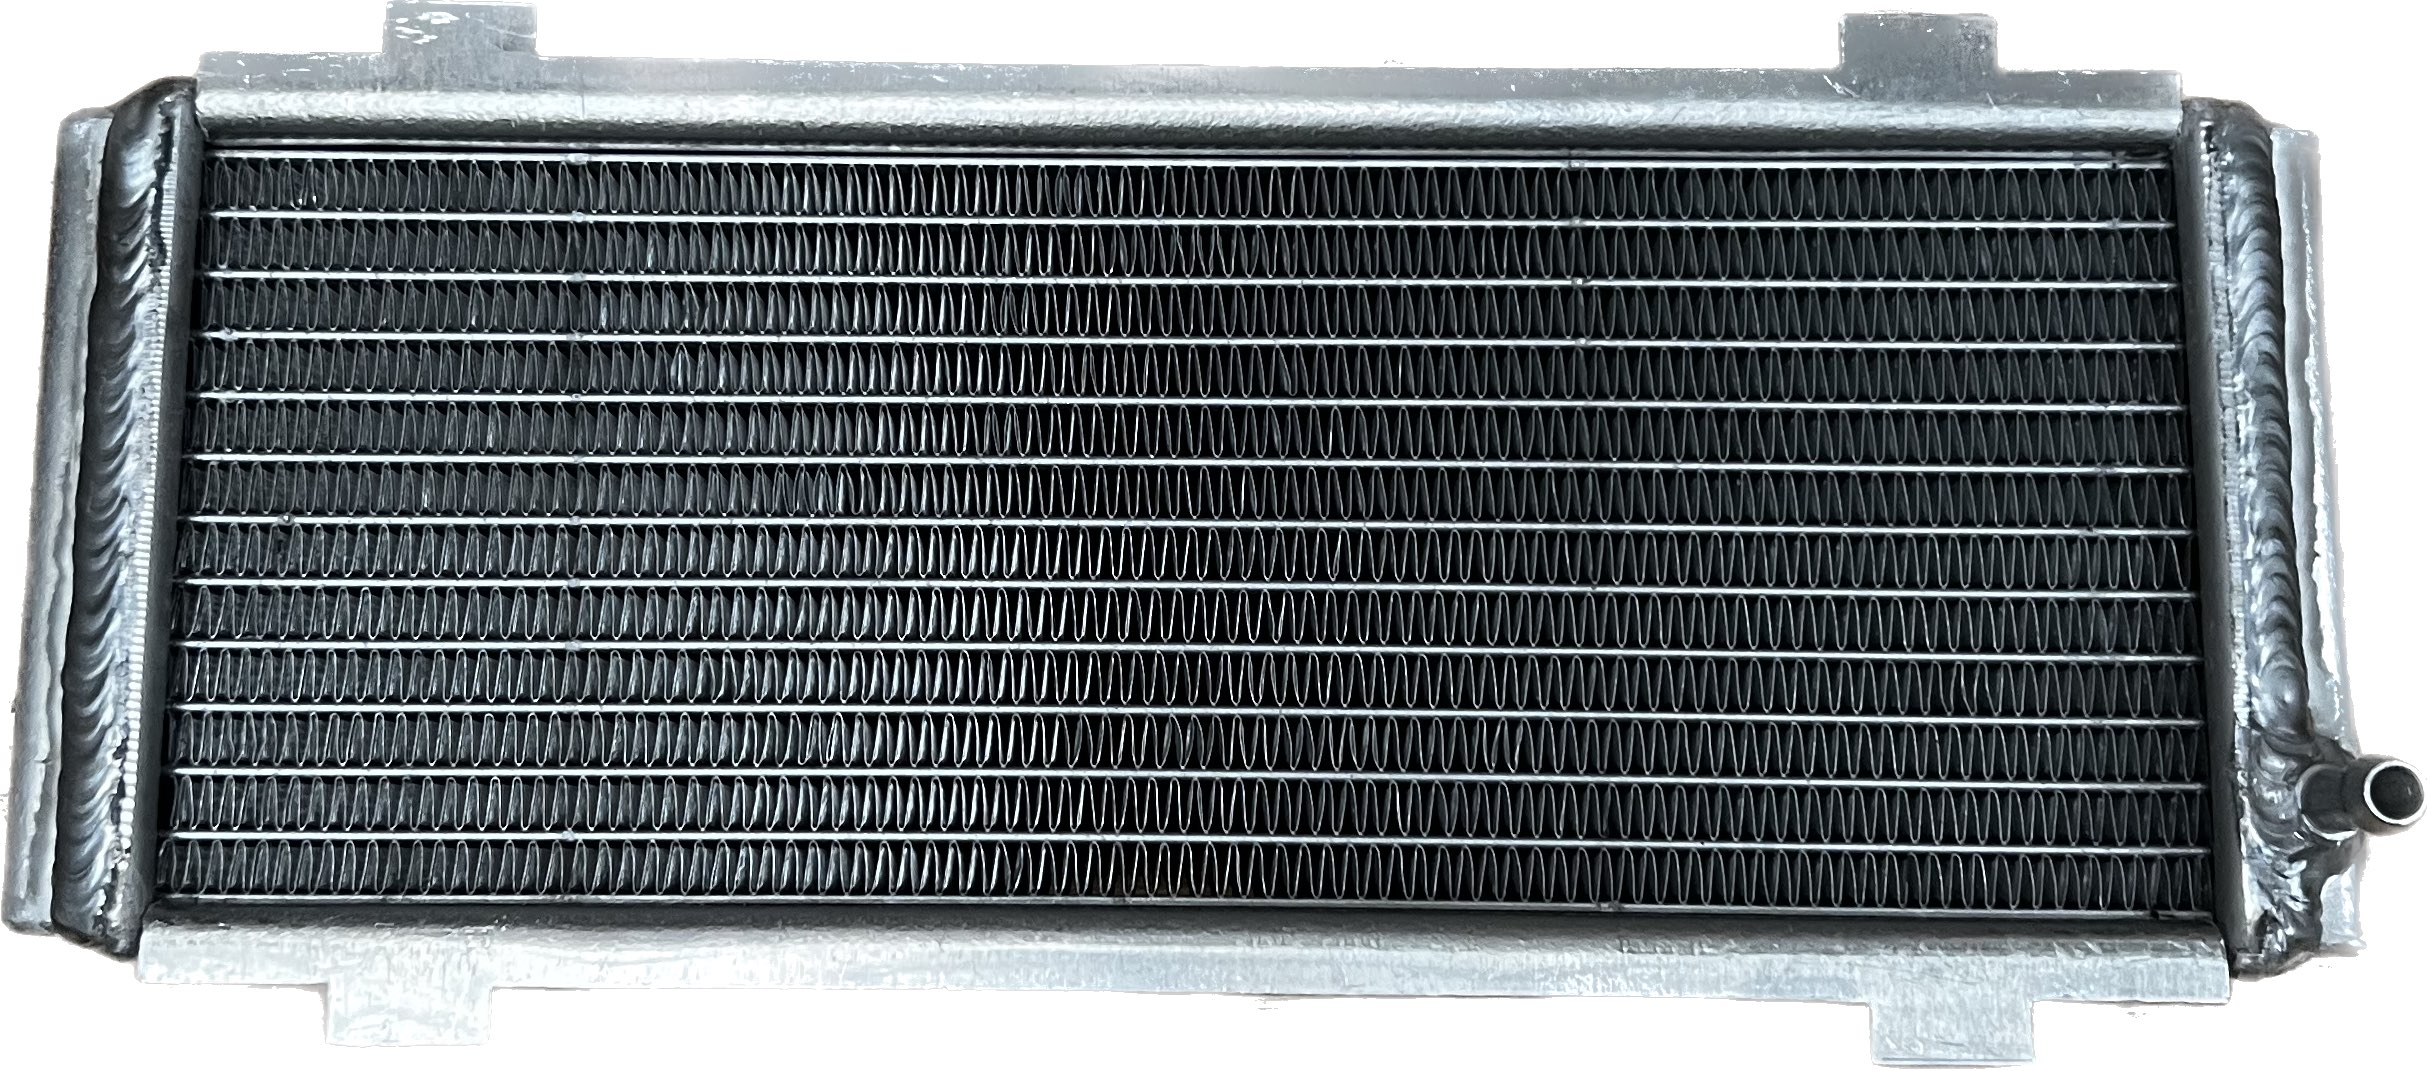
\includegraphics[width=.9\linewidth]{Img/Kapitola1/radiator.jpg}
    %         \caption{V\'{y}m\v{e}n\'{\i}k tepla pou\v{z}it\'{y} pro chlazen\'{\i} FSE.11 v roce 2022. Z archivu autora.}
    %         \label{fig:Radiator_live}
    %     \end{figure}

    \todo[inline]{Turbulence + veliciny}

    \section{Formulace 3D \'{u}lohy}
    \label{sec:DefCas3D}
        
        
        Tato sekce bude v\v{e}nov\'{a}na formulaci 3D \'{u}lohy proud\v{e}n\'{\i} tekutiny. M\v{e}jme tedy 3D oblast tvaru kv\'{a}dru $\Omega = (0,W) \times (0,H) \times (0,H)$, $W,H \in \mathbb{R}^+$, stejnou jako v sekc\'{\i}ch \ref{sec:DesFluDyn} a \ref{sec:HeatTransfer}. \v{C}asov\'{y} interval uva\v{z}ujme $\mathcal{I} = \langle 0,\mathcal{T} \rangle$ pro $\mathcal{T} \in \mathbb{R}^{+}$.
        
        Pro izoterm\'{a}ln\'{\i} syst\'{e}m s nestla\v{c}itelnou, newtonovskou, vazkou tekutinou m\v{e}jme z\'{a}kony zachov\'{a}n\'{\i} ve tvaru 
        \begin{subequations}
        \label{eq:DefCasLaw3}
        \begin{align}
            \sum_{i=1}^{3}\frac{\partial u_i}{\partial x_i} &= 0, \label{eq:DefCasMom3} \\
            \rho \frac{\partial u_i}{\partial t} + \rho \sum_{j=1}^{3}\frac{\partial}{\partial x_j} (u_j u_i) &= \rho \nu \sum_{j=1}^{3}\frac{\partial}{\partial x_j} \left( \frac{\partial u_i}{\partial x_j} + \frac{\partial u_j}{\partial x_i} \right) - \frac{\partial P}{\partial x_i} \qquad \ i \in \{ 1,2,3 \}, \label{eq:DefCasMas3} \\
            \rho \frac{\partial T}{\partial t} &= \nabla \cdot ( \kappa T) - \rho \boldsymbol{u} \cdot \nabla T, \label{eq:DefConPotEne}
        \end{align}    
        \end{subequations}
        na oblasti $\Omega \times \mathcal{I}$, kde $\boldsymbol{u} = (u_1,u_2,u_3)^\intercal$ zna\v{c}\'{\i} vektor rychlosti a $x_i$ jsou po \v{r}ad\v{e} slo\v{z}ky polohov\'{e}ho vektoru $\boldsymbol{x} = (x_1,x_2,x_3)^\intercal$. V\v{s}echny veli\v{c}iny mohou b\'{y}t obecn\v{e} z\'{a}visl\'{e} na poloze $\boldsymbol{x}$, \v{c}ase $t$ a teplot\v{e} $T$. Prvn\'{\i} rovnice odpov\'{\i}d\'{a} rovnici kontinuity \eqref{eq:ConEqu}, druh\'{a} z\'{a}konu zachov\'{a}n\'{\i} hybnosti \eqref{eq:LawConMom} a posledn\'{\i} rovnici veden\'{\i} tepla \eqref{eq:HeaEqu}.
        
        Pro 3D \'{u}lohu zb\'{y}v\'{a} je\v{s}t\v{e} dodefinovat okrajov\'{e} a po\v{c}\'{a}te\v{c}n\'{\i} podm\'{\i}nky. Ty jsou pro \v{r}e\v{s}en\'{\i} Navierov\'{y}ch-Stokesov\'{y}ch rovnic tvaru
        % \begin{pmatrix} \frac{16U_{\infty}}{H^4}(Hx_{2}- {x}_2^2)(Hx_3 - x_3^2) \\ 0 \end{pmatrix}
        \begin{subequations}
        \label{eq:DefCasConNSE3D}
        \begin{align}
        \Big( \nabla p(\boldsymbol{x},t) - \nu \rho \Laplace \boldsymbol{u} \Big) \cdot \boldsymbol{n} &= 0, & \boldsymbol{u} (\boldsymbol{x},t) &= (u_{in}, 0, 0)^\intercal  & &\forall (\boldsymbol{x},t) \in \Gamma_{in} \times \mathcal{I}, \label{eq:DefCasConInl3}\\
            \nabla p(\boldsymbol{x},t) \cdot \boldsymbol{n} &= 0, & \boldsymbol{u} (\boldsymbol{x},t) &= 0 & &\forall (\boldsymbol{x},t) \in \Gamma_{w} \times \mathcal{I}, \label{eq:DefCasConWal3} \\
            p(\boldsymbol{x},t) &= p_{out}(\boldsymbol{x},t), & \nabla u_i (\boldsymbol{x},t) \cdot \boldsymbol{n} &= 0 \ \forall i \in \{ 1,2 \}, & &\forall (\boldsymbol{x},t) \in \Gamma_{out} \times \mathcal{I},  \label{eq:DefCasConOut3} \\
            \nabla p(\boldsymbol{x},t) \cdot \boldsymbol{n} &= 0, & \boldsymbol{u} (\boldsymbol{x},0) &= 0 & &\forall \boldsymbol{x} \in \Omega, \label{eq:DefCasIniCon3}
        \end{align}
        \end{subequations}
        kde $\boldsymbol{u}_{in}$ zna\v{c}\'{\i} rychlost na vstupn\'{\i} \v{c}\'{a}sti hranice $\Gamma_{in}$. Pro \v{r}e\v{s}en\'{\i} advek\v{c}n\v{e}-difuzn\'{\i} \'{u}lohy \eqref{eq:DefConPotEne} jsou okrajov\'{e} a po\v{c}\'{a}te\v{c}n\'{\i} podm\'{\i}nky tvaru
        \begin{subequations}
            \label{eq:DefCasConADE3D}
            \begin{align}
                T (\boldsymbol{x},t) &= T_{in}  & &\forall (\boldsymbol{x},t) \in \Gamma_{in} \times \mathcal{I}, \label{eq:DefCasConInl33}\\
                T (\boldsymbol{x},t) &= 0 & &\forall (\boldsymbol{x},t) \in \Gamma_{w} \times \mathcal{I}, \label{eq:DefCasConWal33} \\
                \nabla T_i (\boldsymbol{x},t) \cdot \boldsymbol{n} &= 0 \ \forall i \in \{ 1,2 \}, & &\forall(\boldsymbol{x},t) \in \Gamma_{out} \times \mathcal{I},  \label{eq:DefCasConOut33} \\
                T (\boldsymbol{x},0) &= T_{a} & &\forall \boldsymbol{x} \in \Omega \backslash \overline{\Omega}_{b}, \label{eq:DefCasIniCon33} \\
                T (\boldsymbol{x},0) &= T_b & &\forall(\boldsymbol{x},t) \in \overline{\Omega}_{b} \times \mathcal{I},  \label{eq:DefCasConOut333} \\
                \boldsymbol{J}_{a}(\boldsymbol{x}, t) \cdot \boldsymbol{n}_v &= \mathrm{Sh}\,( T_v(\boldsymbol{x},t) - T_b(\boldsymbol{x},t)) & &\forall (\boldsymbol{x}, t) \in \Gamma_{b} \times \mathcal{I}, \label{eq:DefCasIniConFloa} \\
                \boldsymbol{J}_{b}(\boldsymbol{x}, t) \cdot \boldsymbol{n}_b &= \mathrm{Sh} \,( T_b(\boldsymbol{x},t) - T_v(\boldsymbol{x},t)) & &\forall (\boldsymbol{x}, t) \in \Gamma_{b} \times \mathcal{I}, \label{eq:DefCasIniConFlob} 
            \end{align}
            \end{subequations}
            kde $T_{in}$ zna\v{c}\'{\i} teplotu na vstupn\'{\i} \v{c}\'{a}sti oblasti, $T_{v}$ je po\v{c}\'{a}te\v{c}n\'{\i} teplota v oblasti mimo p\v{r}ek\'{a}\v{z}ku a $T_{b}$ zna\v{c}\'{\i} po\v{c}\'{a}te\v{c}n\'{\i} teplotu na p\v{r}ek\'{a}\v{z}ce. Rovnice \eqref{eq:DefCasIniConFloa} resp. \eqref{eq:DefCasIniConFlob} odpov\'{\i}daj\'{\i} tepeln\'{e}mu toku z oblasti do t\v{e}lesa resp. z t\v{e}lesa do oblasti, viz \cite{mika1999chemicke}. 

            P\v{r}i \v{r}e\v{s}en\'{\i} \'{u}lohy budeme uva\v{z}ovat r\r{u}zn\'{e} hodnoty difuzn\'{\i}ho koeficientu v z\'{a}vislosti na poloze, tj. $D = D(\boldsymbol{x})$. V p\v{r}\'{\i}pad\v{e}, \v{z}e se budeme nach\'{a}zet na t\v{e}lese $\Omega_b$, uva\v{z}ujeme difuzn\'{\i} koeficient s ozna\v{c}en\'{\i}m $D_b$. V opa\v{c}n\'{e}m p\v{r}\'{\i}pad\v{e} jej budeme zna\v{c}it $D_a$.
        
        % Pro~korektnost zm\'{\i}n\'{\i}me, \v{z}e parabolick\'{y} profil ur\v{c}en\'{y} vztahem \eqref{eq:DefCasConInl3} nen\'{\i} konzistentn\'{\i} s p\v{r}esn\'{y}m \v{r}e\v{s}en\'{\i}m pro~proud\v{e}n\'{\i} v oblasti s obecn\v{e} obd\'{e}ln\'{\i}kov\'{y}m pr\r{u}\v{r}ezem. Spr\'{a}vn\'{e} \v{r}e\v{s}en\'{\i} bychom na\v{s}li za pomoci nekone\v{c}n\'{e} Fourierovy \v{r}ady, viz \cite{white2006viscous}. V\'{y}raz $\nu \rho \Laplace \boldsymbol{u}$ je pro podm\'{\i}nky \eqref{eq:DefCasConWal3}, \eqref{eq:DefCasConOut3} a \eqref{eq:DefCasIniCon3} nulov\'{y}.
